% !TeX program = xelatex
% Compile twice with XeLaTeX. Figures are in figures/ (standalone) or ../figures/ (project).
\documentclass[12pt,a4paper]{article}
\usepackage{fontspec}
\usepackage{polyglossia}
\setdefaultlanguage{russian}
\setotherlanguage{english}
\setmainfont{DejaVu Serif}
\setsansfont{DejaVu Sans}
\setmonofont{DejaVu Sans Mono}
\usepackage{amsmath,amssymb,amsthm,mathtools}
\usepackage[a4paper,left=24mm,right=24mm,top=23mm,bottom=24mm]{geometry}
\usepackage{graphicx,booktabs,tabularx,array,float,caption}
\usepackage{enumitem,fancyhdr,xcolor,xurl,hyperref}
\graphicspath{{figures/}{../figures/}}
\definecolor{inkblue}{HTML}{234D65}
\hypersetup{colorlinks=true,linkcolor=inkblue,urlcolor=inkblue,citecolor=inkblue,pdftitle={Пространственная конкуренция фитнес-клубов Марьино}}
\setlength{\parindent}{1.1em}
\setlength{\parskip}{3pt}
\setlength{\headheight}{15pt}
\pagestyle{fancy}
\fancyhf{}\fancyhead[L]{\small\sffamily РЭШ / Микроэкономика}\fancyhead[R]{\small\sffamily Марьино}
\fancyfoot[C]{\small\thepage}
\renewcommand{\headrulewidth}{0.3pt}
\captionsetup{font=small,labelfont=bf}
\setlist{nosep,leftmargin=*}
\renewcommand{\arraystretch}{1.15}
\newcolumntype{Y}{>{\raggedright\arraybackslash}X}
\newcommand{\one}{\mathbf{1}}
\newcommand{\dd}{\mathrm{d}}
\newcommand{\argmax}{\operatorname*{arg\,max}}
\newcommand{\argmin}{\operatorname*{arg\,min}}
\newcommand{\rub}{\text{руб.}}
\newcommand{\PP}{\text{п.п.}}
\newtheorem{proposition}{Утверждение}
\allowdisplaybreaks[2]
\emergencystretch=2em
\begin{document}
\begin{titlepage}
\thispagestyle{empty}
\begin{center}
{\large Российская экономическая школа\par}
{\large Курс микроэкономики\par}
\vspace{2cm}
{\LARGE\bfseries Пространственная конкуренция\par фитнес-клубов района Марьино\par}
\vspace{.5cm}
{\large Каннибализация, ограничения размещения\par и стратегия расширения DDX Fitness\par}
\vspace{1.4cm}
\end{center}
\noindent Команда: \rule{.72\linewidth}{.4pt}\\[8pt]
Участники: \rule{.67\linewidth}{.4pt}
\vspace{1cm}
\begin{center}\textbf{Аннотация}\end{center}
Исследуется рынок потенциального спроса жителей Марьино. Сетевая модель Хотеллинга с пешеходными расстояниями и неоднородной плотностью населения позволяет оценить каннибализацию, наилучшие ответы и выгодность перемещения существующих клубов. Множество стратегий ограничивается наблюдаемыми коммерческими зданиями OpenStreetMap, а не обучаемым рейтингом. На основном наборе из 34 потенциальных площадок средний сетевой выигрыш от переезда сокращается с 7,21 до 4,91 п.п., но максимальный остаётся 11,90 п.п. Жилые веса уточнены по числу квартир (361 из 365 объектов сопоставлены). При фиксированных тарифах и альтернативных моделях спроса меняются равновесия и пороги безубыточности. Рекомендуется искать помещения в восточной части района и принимать решение об открытии после проверки конкретного договора аренды. Дополнительно сопоставлены рейтинги и даты открытия девяти клубов, рассчитаны коэффициенты переключения спроса и исследовано расхождение для DDX «Люблю Молл». Наблюдаемые объёмы продаж и параметры предпочтений отсутствуют; оценки сценарные.
\par\medskip\noindent\textbf{Ключевые слова:} Хотеллинг, пространственная конкуренция, равновесие Нэша, каннибализация, коммерческая недвижимость.
\vfill\begin{center}Ноябрь 2026 г.\end{center}
\end{titlepage}
\tableofcontents
\clearpage
\section{Рынок и исходные данные}
Фитнес --- пространственно дифференцированная услуга: потребитель регулярно несёт транспортные издержки, а фирмы выбирают не только тарифы и сервис, но и расположение. Цель работы --- оценить, насколько существующее размещение клубов Марьино согласуется с теорией пространственной конкуренции, и обосновать стратегию DDX. Рассматривается спрос жителей района, а не вся клиентская база московских сетей. Внешние клубы могут конкурировать за этих жителей.

В архивном снимке OSM имеются 365 жилых объектов, 23 клуба 18 сетей (девять внутри района), матрицы расстояний до существующих клубов и 3894 географических точек сетки с шагом 50 м. Исходная оценка весов жилых объектов использует площадь основания $S_i$ и этажность $h_i$. Основная уточнённая оценка использует число квартир $n_i$:
\begin{equation}
 w_i^{(0)}=P\frac{S_ih_i}{\sum_k S_kh_k},\qquad w_i=P\frac{n_i}{\sum_k n_k},\qquad P=273463.
\end{equation}
Вторичный жилищный справочник «Домпаспорт» содержит 358 собранных адресных записей (87209 квартир); сопоставлены 355 адресов, или 361 из 365 объектов OSM (86759 квартир). Если одному адресу соответствуют несколько контуров, число квартир делится пропорционально $S_i h_i$, без двойного счёта. Для четырёх оставшихся объектов число квартир оценено через отношение суммы квартир к сумме $S_i h_i$ по сопоставленным объектам. На них приходится 1,38\% итогового веса. Численность 273463 согласуется с опубликованным вторичным воспроизведением статистики населения района на 01.01.2025; первичная таблица Мосстата напрямую не получена. Число квартир не измеряет фактическую заселённость. Первичный реестр ГИС ЖКХ не выгружен. Прежние веса сохранены как контрольный сценарий. Пешеходное время $t_{ij}=d_{ij}/80$ минут, где $d_{ij}$ --- архивное расстояние по графу OSM в метрах с отрезками привязки. Матрицы используются без повторной загрузки графа.
\begin{figure}[H]\centering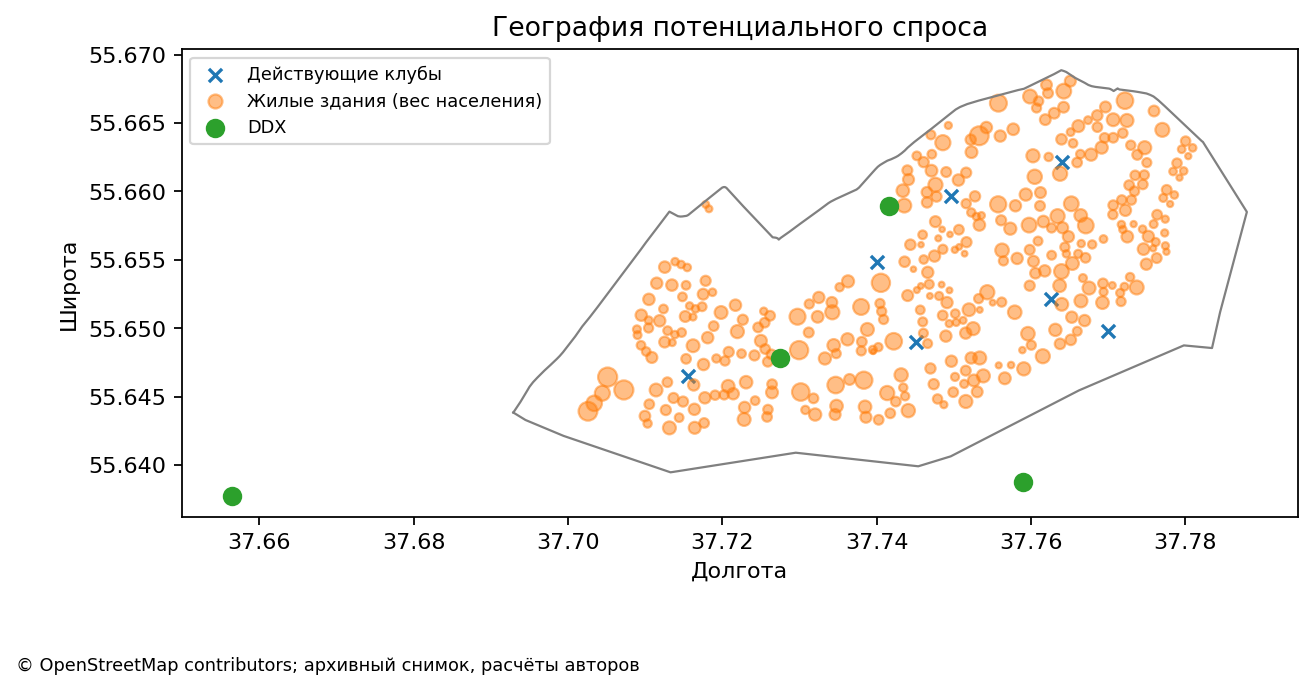
\includegraphics[width=.92\linewidth]{market.png}\caption{Жилые объекты и существующие клубы. Размер метки жилья отражает вес спроса.}\end{figure}
\subsection{Рыночная структура}
Наблюдаемые продажи недоступны. Для сравнения трёх вложенных определений рынка используем модельные доли потенциального спроса $s_A$. Индексы $HHI=\sum_A(100s_A)^2$ и $CR_3=100\sum_{k=1}^3s_{(k)}$ характеризуют концентрацию только в рамках принятой модели. $s_{(k)}$ --- доли по убыванию.
\begin{table}[H]\centering\caption{Концентрация в базовой модели}\begin{tabular}{lrrrrr}\toprule Рынок & Клубы & Сети & HHI & CR3, \% & DDX, \%\\\midrule Узкий & 8 & 4 & 5051 & 100,00 & 55,68\\ Расширенный & 13 & 9 & 3011 & 85,64 & 14,20\\ Широкий & 23 & 18 & 1466 & 54,54 & 13,07\\\bottomrule\end{tabular}\end{table}
Различие между сегментами принципиально: бассейн, СПА, доступ в сеть, групповые занятия и режим работы делают клубы неоднородными. Архивные месячные тарифы DDX (Smart, 2400 руб.), Spirit (2600), Академии Спорта (2590), Fitnation (1990), XFIT (2990) Magneto (от 3742) и Kometa (3700, продление по прайсу от 01.09.2026) не образуют полной выборки одинаковых продуктов. Стоимость подписок, промоакции и вступительные платежи требуют оговорок. Дополнительные издержки входа включают аренду, ремонт, оборудование, инженерные требования и операционные расходы. Семь внешних записей реестра требуют актуализации. Их совместное исключение не меняет базовый широкий результат: ни одна не является ближайшей для положительной массы спроса. Дополнительно выявлен женский клуб «Мисс Фитнес» (Новочеркасский б-р, 44); он не включён в основной универсальный сегмент, но его здание исключено из консервативного набора площадок. При условном включении этого клуба как универсального (расстояния по ближайшей сохранённой точке) доля DDX падает до 9,42\%, а оптимум и прирост 12,85 п.п. сохраняются. YoBody и архивная Территория фитнеса фигурируют по одному адресу; второй объект не добавлен без подтверждения. Закрытый XFIT Марьино не следует смешивать с XFIT Point Люблинский парк. Полного нового реестра нет.

\subsection{Локальная доступность}
Пусть $n_i(r)=\sum_A\one\{\min_{j\in J_A}t_{ij}\le r\}$ --- число сетей в пределах $r$ минут пешком. Доля населения с ровно одной доступной сетью равна $\sum_iw_i\one\{n_i(r)=1\}/P$. При $r=10$ минут она составляет 57,55\%; 26,39\% не имеют ни одной сети в этом радиусе, а 16,05\% имеют две или более. При $r=15$ минут две или более сети доступны уже 71,28\%. Это ограниченность выбора в заданном радиусе, а не доказанная локальная монополия.
\begin{figure}[H]\centering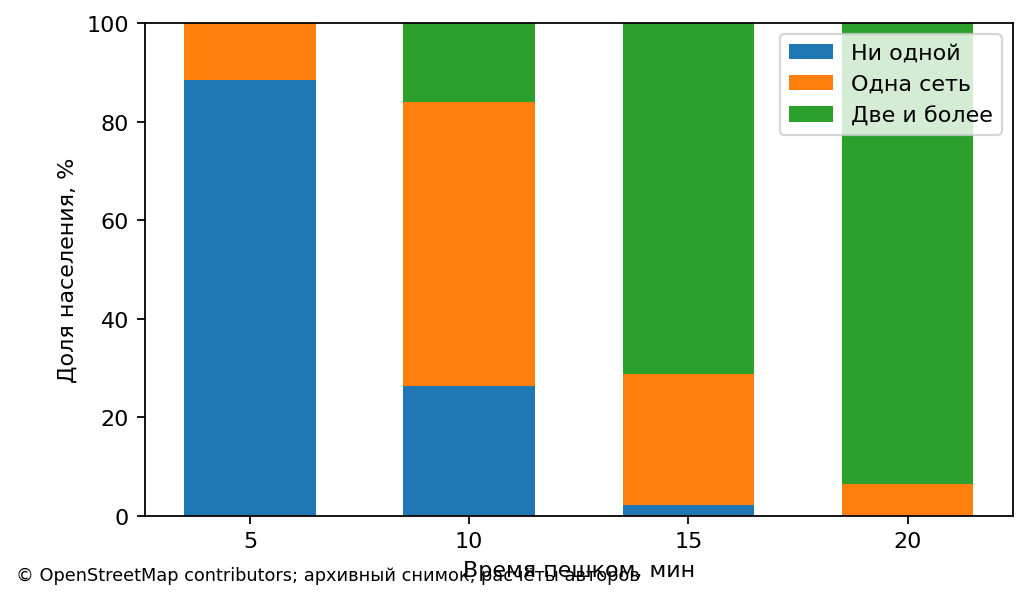
\includegraphics[width=.77\linewidth]{overlap.png}\caption{Локальная доступность сетей на широком рынке.}\end{figure}
\section{Математическая модель пространственного выбора}
\subsection{Потребители, фирмы и спрос}
Пусть $I=\{1,\ldots,N\}$ --- жилые объекты, $J$ --- клубы, $\mathcal A$ --- фирмы, $a(j)$ --- владелец клуба и $J_A=\{j:a(j)=A\}$. Конфигурация рынка $l=(l_j)_{j\in J}$. В базовой модели одинаковы цена, качество и положительная маржа всех клубов. При условии покупки абонемента потребитель максимизирует $U_{ij}=v-p-\tau t_{ij}(l_j)$, $\tau>0$. Поэтому
\begin{align}
 M_i(l)&=\argmin_{j\in J}t_{ij}(l_j),\\
 \pi_{ij}(l)&=\frac{\one\{j\in M_i(l)\}}{|M_i(l)|},\\
 D_j(l)&=\sum_iw_i\pi_{ij}(l),\quad D_A(l)=\sum_{j\in J_A}D_j(l),\quad s_A(l)=D_A(l)/P.
\end{align}
При точном равенстве расстояний спрос делится поровну между клубами. Сумма $\sum_A D_A=P$. Если доля покупающих абонементы $\theta$, то число абонементов в модели $Q_A=\theta D_A$. В базовом анализе размещения фиксированные затраты одинаковы по локациям и максимизация $D_A$ эквивалентна максимизации маржинальной прибыли. Никаких параметров потребительского выбора из цен не оценивается.
\subsection{Открытие и каннибализация}
Для кандидата $z$ определим $d_i=\min_jt_{ij}$, $k_i=|M_i|$, $a_{iA}=\sum_{j\in J_A}\pi_{ij}$. Доля спроса объекта $i$, перетекающая в новый клуб:
\begin{equation}
 b_i(z)=\begin{cases}1,&t_{iz}<d_i,\\1/(k_i+1),&t_{iz}=d_i,\\0,&t_{iz}>d_i.\end{cases}
\end{equation}
Валовой спрос новой точки $G(z)=\sum_iw_ib_i(z)$; каннибализация $C_A(z)=\sum_iw_ib_i(z)a_{iA}$. Тогда чистый прирост сети
\begin{equation}
 \Delta D_A(z)=\sum_iw_ib_i(z)(1-a_{iA})=G(z)-C_A(z).
\end{equation}
Доказательство: в объекте $i$ после открытия остаётся доля $1-b_i$ прежнего спроса и добавляется доля $b_i$ нового клуба. Суммарная доля фирмы становится $(1-b_i)a_{iA}+b_i$, откуда результат. Если $z_0$ максимизирует $G$ и $C_A(z_0)=0$, то $\Delta D_A(z)\le G(z)\le G(z_0)=\Delta D_A(z_0)$ для любой $z$. Общий оптимум разных фирм возможен; различия возникают из-за собственных действующих точек.
\section{Реалистичное множество стратегий}
\subsection{Правило отбора}
Используем адресный полигональный слой OSM из исходного архива: 5782 полигона, 920 с репрезентативной точкой внутри района, 103 с тегами \texttt{retail} или \texttt{commercial} (допускается также \texttt{sports\_centre}, но таких записей в слое нет). Это адресный слой, не полный реестр зданий. Площадь $S_b$ измеряется в проекции UTM 37N (EPSG:32637). Для здания $b$ репрезентативная внутренняя точка привязывается к ближайшей допустимой точке $g(b)$ прежней сетки $L_0$. Расстояние привязки $r_b$ ограничивается 200 м. Расстояние $d_b$ от контура до ближайшего известного клуба рассчитывается в той же проекции. Основной сценарий:
\begin{equation}
 L(S)=\{g(b): b\text{ коммерческое},\ S_b\ge S,\ r_b\le200,\ d_b>30,\ b\notin B_{\rm known}\}.
\end{equation}
Порог 1100 м$^2$ ориентирован на опубликованные требования DDX Basic (площадь помещения 1100--1500 м$^2$, высота под коммуникациями от 4 м). Площадь контура --- грубый индикатор потенциального размера помещения; этажность, свободные блоки, высота и конструктивная пригодность неизвестны. В $B_{\rm known}$ включён выявленный контур женского клуба (OSM 46679150). Отсечение 30 м --- консервативный сценарный запрет на потенциально занятые здания, не факт отсутствия свободного блока. Проверяем также включение таких зданий. Порог одинаков для сетей только ради сравнимости, реальные форматы различаются.
\begin{table}[H]\centering\caption{Множества стратегий}\begin{tabular}{lrr}\toprule Условие & Здания & Точки\\\midrule Сетка $L_0$ & --- & 3894\\ $S\ge500$ & 69 & 66\\ $S\ge1100$ & 34 & 34\\ $S\ge1500$ & 18 & 18\\ $S\ge1100$, включая занятые прокси & 40 & 40\\\bottomrule\end{tabular}\end{table}
\begin{figure}[H]\centering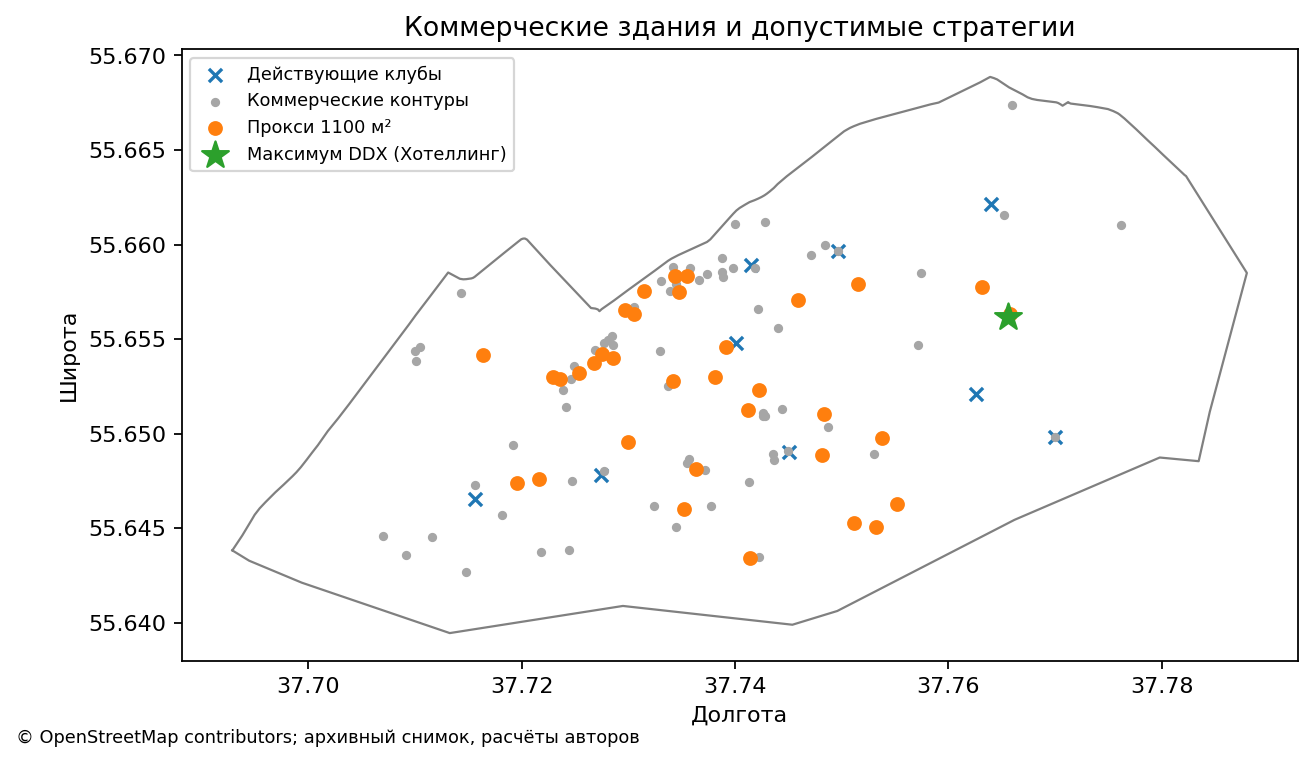
\includegraphics[width=.93\linewidth]{buildings.png}\caption{Отбор потенциальных площадок. Звезда --- оптимум DDX в базовой модели.}\end{figure}
\subsection{Оптимизация расширения}
Для каждого рынка $m$ и фирмы $A$ решаем $\max_{z\in L}\Delta D_A^m(z)$. Для DDX дополнительно вычисляем $\argmax_{z\in L}\min_m 100\Delta D_A^m(z)/P$. Это максимизация гарантированного прироста по трём определениям рынка, а не вероятность сценария.
\begin{table}[H]\centering\caption{Робастный оптимум DDX, прирост доли в п.п.}\begin{tabularx}{\linewidth}{Yrrr}\toprule Множество & Узкий & Расширенный & Широкий\\\midrule Сетка, восточная точка & 21,48 & 32,57 & 15,55\\ Коммерческие площадки 1100 м$^2$ & 23,56 & 30,00 & 12,85\\\bottomrule\end{tabularx}\end{table}
Робастный оптимум на основном наборе соответствует контуру Новомарьинская ул., 20 (OSM way/51675639, площадь 1503 м$^2$, привязка около 20 м). Та же точка максимизирует прирост на широком рынке. На полной сетке общий оптимум имеют 15 из 18 фирм; в основном наборе 16 фирм выбирают один узел, однако их чистый прирост различается вследствие каннибализации. Magneto и Территория фитнеса выбирают ул. Маршала Голованова, 5. При старых весах населения оптимум DDX на основном наборе также соответствовал Новомарьинской, 20; прирост был 14,20 п.п. вместо 12,85. На широком рынке HHI изменился с 1412 до 1466, доля DDX --- с 10,93 до 13,07\%. Полные таблицы по всем фирмам и рынкам в \texttt{results/optima.csv}, сравнение весов в \texttt{population\_comparison.csv}.
\section{Равновесие и фактическое размещение}
\subsection{Односторонние перемещения}
В конфигурации $l^0$ фирма может сохранить положение или переместить один из своих клубов внутри района, не меняя другие локации. Пусть $J_A^{\rm in}$ --- множество таких клубов. Определим выигрыш в п.п.:
\begin{align}
 R_{Aj}(L)&=\max\left(0,\max_{z\in L}\frac{100[D_A(l^0_{-j},z)-D_A(l^0)]}{P}\right),\\
 R_A(L)&=\max_{j\in J_A^{\rm in}}R_{Aj}(L),\quad \epsilon(L)=\max_A R_A(L).
\end{align}
Точное равновесие относительно рассматриваемых одноклубных отклонений требует $\epsilon=0$. Средний regret --- описательная статистика, не критерий равновесия. Если $L_1\subseteq L_2$, то $R_A(L_1)\le R_A(L_2)$; уменьшение regret от сокращения множества стратегий закономерно и не доказывает правильность фильтра.
\begin{table}[H]\centering\caption{Регрет фактической конфигурации, п.п.}\begin{tabular}{lrr}\toprule Сеть & Сетка & Здания от 1100 м$^2$\\\midrule Spirit & 1,86 & 0,00\\ Территория фитнеса & 2,71 & 0,00\\ Академия Спорта & 4,72 & 2,01\\ Z Fitness & 6,96 & 3,50\\ Magneto & 6,54 & 5,62\\ Kometa & 9,61 & 8,30\\ СССР & 10,69 & 7,98\\ DDX & 14,61 & 11,90\\\midrule Среднее по восьми сетям & 7,21 & 4,91\\ Максимум & 14,61 & 11,90\\\bottomrule\end{tabular}\end{table}
\begin{figure}[H]\centering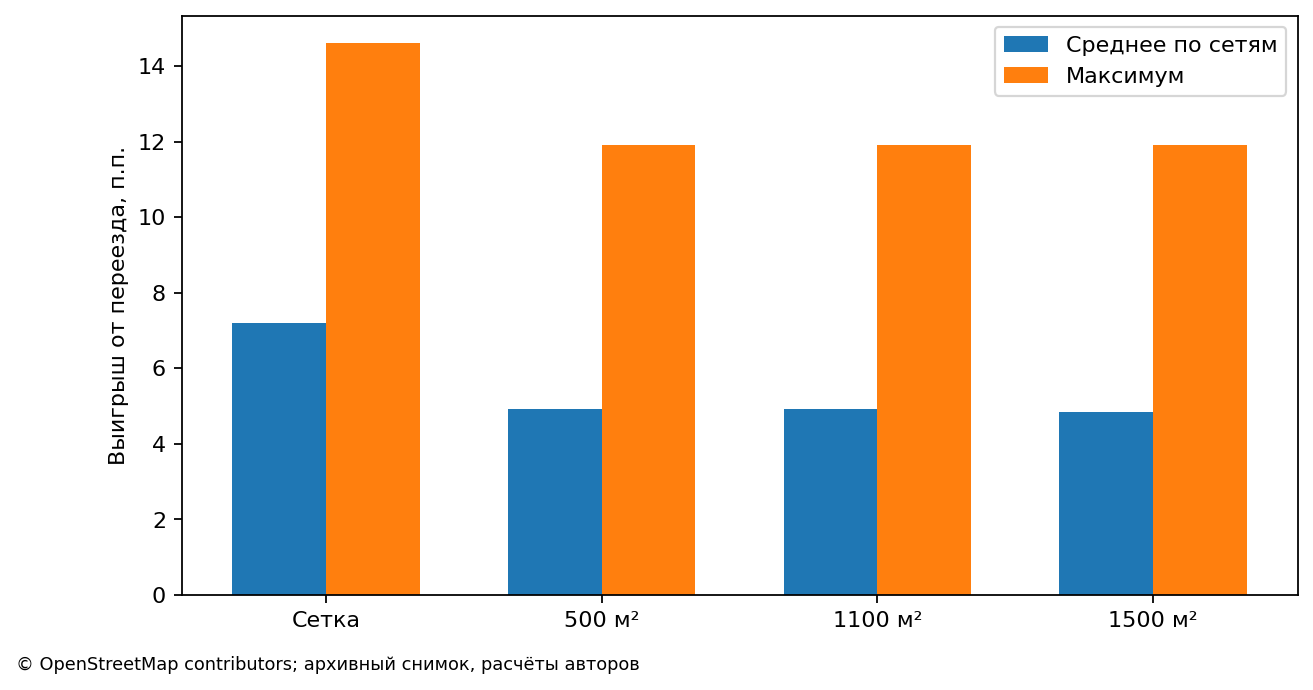
\includegraphics[width=.85\linewidth]{regret.png}\caption{Чувствительность регрета к ограничениям стратегий.}\end{figure}
Для Spirit и Территории фитнеса ни одна из 34 альтернатив не улучшает спрос. Для DDX лучший найденный переезд «Люблю Молл» даёт 11,90 п.п. Включение шести потенциально занятых коммерческих зданий не меняет максимумы. Рынок в целом не является точным равновесием данной игры. При издержках переезда $K_{Aj}(z)$ условие выгодного отклонения меняется на $m_A\theta[D_A(l^0_{-j},z)-D_A(l^0)]>K_{Aj}(z)$. Договоры аренды и издержки перемещения неизвестны.
\subsection{Ретроспективная проверка локаций}
Временно удалим клуб $j$ и сравним его фактический чистый вклад $d_j=D_A(l^0)-D_A(l^0_{-j})$ с лучшим модельным вкладом
\[d_j^*=\max\left(d_j,\max_{z\in L}\Delta D_A(l^0_{-j},z)\right).\]
Отношение $e_j=d_j/d_j^*$ при $d_j^*>0$ измеряет долю реализуемого выигрыша. Оно дополняет regret, но не является независимой проверкой: $R_{Aj}=100(d_j^*-d_j)/P$. Медиана по девяти клубам на основном наборе --- 74,5\%, среднее --- 67,0\%. Spirit и Территория фитнеса достигают 100\%, DDX Экран --- 84,7\%, DDX Люблю Молл --- 7,4\%. Это не исторический прогноз: инфраструктура и остальные клубы зафиксированы в текущем снимке, а не на дату открытия. Результаты для обоих способов взвешивания в \texttt{loo.csv}.
\subsection{Одновременная игра DDX и Spirit}
Сети одновременно открывают по одному клубу, остальные локации фиксированы. Выигрыш $u_A(x,y)=100[D_A(l^0,x,y)-D_A(l^0)]/P$ и аналогично $u_B$. Равновесие $(x^*,y^*)$ удовлетворяет
\begin{equation}
 x^*\in\argmax_{x\in L}u_A(x,y^*),\qquad y^*\in\argmax_{y\in L}u_B(x^*,y).
\end{equation}
При запрете общей точки множество отклонений зависит от выбора конкурента; это обобщённое равновесие. Для 34 точек перебираются все $34^2$ исходов и все односторонние отклонения. На прежней сетке отдельно проверены две ранее найденные пары (восток--запад и запад--восток); обе при новых весах допускают выгодное отклонение на 1,66 п.п. Это проверка прежних кандидатов, а не новый исчерпывающий поиск на сетке.
\begin{table}[H]\centering\caption{Равновесия на основном наборе площадок}\small\begin{tabularx}{\linewidth}{YYrr}\toprule DDX & Spirit & $u_A$ & $u_B$\\\midrule Марьинский б-р, 7 & Новомарьинская, 20 & 7,73 & 7,48\\ Новомарьинская, 20 & Марш. Голованова, 5 & 5,58 & 8,40\\\bottomrule\end{tabularx}\end{table}
Оба исхода являются равновесиями при разрешённой общей точке и при её запрете. Расстояния между точками 1,03 и 2,36 км. На наборах 66, 34 и 18 точек найдено по два равновесия (при обоих вариантах разрешения общей точки). Ограничения и распределение спроса меняют стратегические исходы. Это не равновесие всей 18-фирменной игры.
\section{Проверка предпосылок спроса}
Базовая модель игнорирует ценовую дифференциацию. Чтобы отделить её эффект от эффекта вероятностного выбора, сравним три правила на одном наборе площадок и при фиксированном общем числе покупателей. Введём приведённые издержки $g_{ij}=t_{ij}+p_{a(j)}/\tau$, где $\tau$ измеряется в рублях месячной цены на минуту времени в одну сторону. В первом варианте минимизируется только $t$, во втором --- $g$. Третий вариант допускает ненаблюдаемую неоднородность предпочтений:
\begin{equation}
 \pi_{ij}=\frac{\exp(-\gamma g_{ij})}{\sum_{k\in J}\exp(-\gamma g_{ik})},\qquad \gamma=\ln2/h.
\end{equation}
$h$ --- период полураспада веса привлекательности по времени. При $h\to0$ Logit стремится к детерминированному выбору минимальных приведённых издержек (при ничьих --- равномерное деление). Это лишь проверка чувствительности, не обученная модель. В отличие от прежних версий, нет перегруженности, эндогенного выбора цен и вложенных моделей. Известные цены сохранены, пропуски заменяются 2000, 2500 или 3000 руб.; $\tau\in\{50,100,200\}$ и $h\in\{5,10,20\}$ минут. Рекламные нижние границы используются условно. Данные не позволяют выбрать истинные параметры.
\begin{table}[H]\centering\caption{Одновременная игра на 34 точках (пропуски 2500 руб., $\tau=100$, $h=10$)}\small\begin{tabularx}{\linewidth}{Yrrr}\toprule Правило выбора & Равновесий без запрета & Расстояние, км & С запретом\\\midrule Ближайший клуб & 2 & 1,03; 2,36 & 2\\ Цена + дорога & 1 & 3,05 & 1\\ Logit & 1 & 0 & 2\\\bottomrule\end{tabularx}\end{table}
При Logit без запрета обе сети выбирают Братиславскую ул., 21 к2; при запрете расстояние 250 м. Следовательно, дифференциация не универсальна даже с ограничением коммерческих площадок. В 27 сценариях Logit на основном наборе оптимумы DDX распределены по трём площадкам (10, 9 и 8 сценариев); в 9 детерминированных ценовых сценариях основной оптимум Новомарьинская, 20 встречается 6 раз. Полные таблицы приведены в CSV. Не следует объявлять одну из спецификаций эмпирически верной. Основной моделью остаётся ближайший клуб; Logit лишь показывает, где результат чувствителен к предпосылке о строгом выборе.
\begin{figure}[H]\centering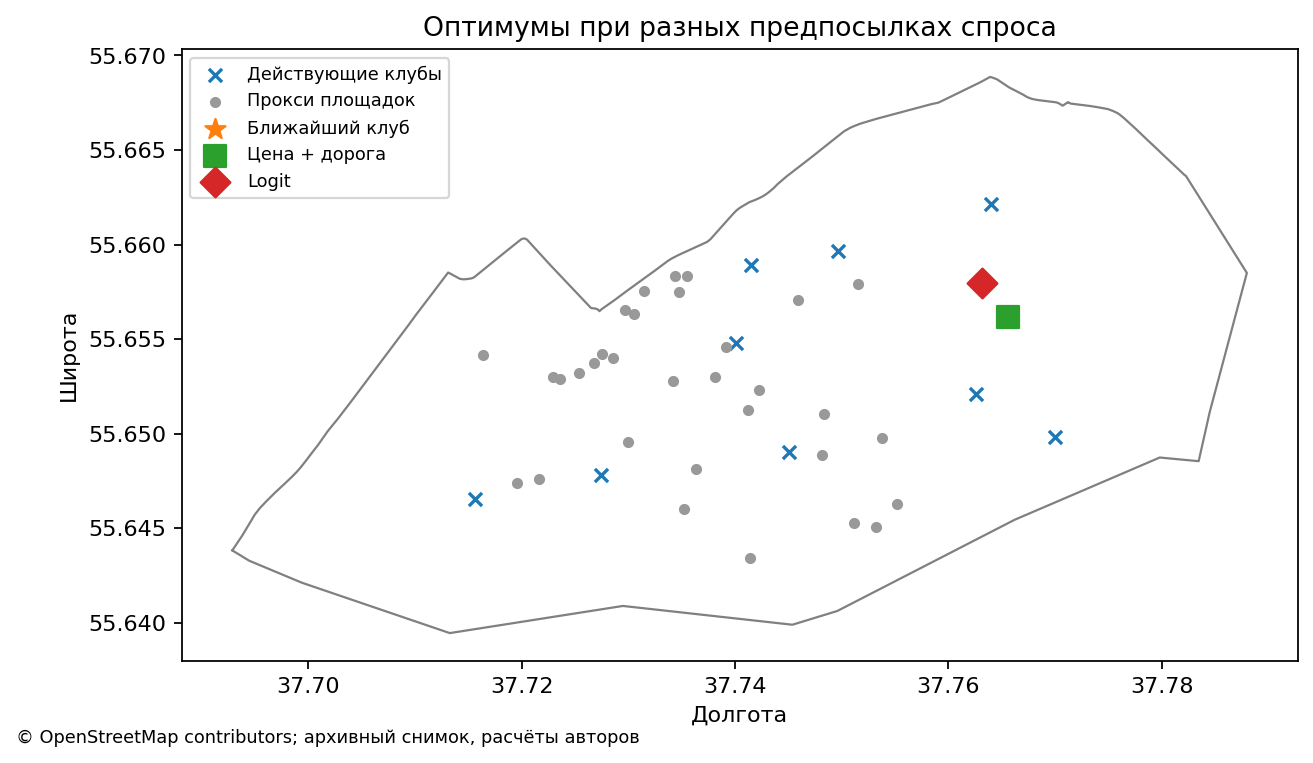
\includegraphics[width=.90\linewidth]{demand.png}\caption{Оптимумы трёх сценариев спроса на одном множестве стратегий.}\end{figure}
\section{Эмпирические объяснения фактического размещения}
\subsection{Цена, качество и локальная конкуренция}
В центральных сценариях (неизвестные тарифы 2500 руб., $\tau=100$, $h=10$) используем опубликованные цены, но они не обязательно соответствуют среднему платежу клиента. В частности, DDX Smart (2400 руб.) выбран по снимку тарифов пользователя и архивным страницам обоих клубов; Light (1900 руб.) оставлен как старый сценарий. Magneto публикует нижнюю границу 3742 руб. Цены и доступность тарифов могут отличаться по клубам. Остальные опубликованные ориентиры: Spirit --- 2600 руб. (предложение до 30.11.2026), Академия Спорта --- 2590, Fitnation --- 1990, XFIT --- 2990, Kometa --- 3700. Источники и оговорки приведены в реестре тарифов.
\begin{table}[H]\centering\caption{Модельные доли спроса при разных правилах выбора, \%}\small\begin{tabularx}{\linewidth}{Yrrr}\toprule Сеть & Ближайший клуб & Цена + дорога & Logit\\\midrule DDX & 13,07 & 14,78 & 21,13\\ Spirit & 14,82 & 18,11 & 9,78\\ Magneto & 10,63 & 1,23 & 4,49\\ Kometa & 6,21 & 2,39 & 3,58\\ Академия Спорта & 18,01 & 16,59 & 9,07\\\bottomrule\end{tabularx}\end{table}
Разница цен DDX и Magneto равна 1342 руб., что в центральном сценарии эквивалентно 13,42 минуты пути. При этом Magneto предоставляет бассейн и СПА, а площадь клуба составляет около 4000 м$^2$. Нельзя отождествлять разницу цены с чистым недостатком полезности. В диагностическом сценарии с ценностью бассейна $b$ вместо $g_{ij}$ используется $g_{ij}-b B_j/\tau$, где $B_j$ --- индикатор подтверждённого бассейна. При $b=1000$ руб. модельная доля Magneto возрастает до 5,52\% (детерминированная модель) или 6,68\% (Logit). Это не оценка готовности платить, а иллюстрация влияния ненаблюдаемого качества.

Сценарный тариф самой DDX также важен: при 1900, 2400 и 2800 руб. модельная доля составляет соответственно 32,18, 14,78 и 8,15\% в модели «цена + дорога»; в Logit --- 27,08, 21,13 и 17,07\%. Вероятностный выбор сглаживает дискретные переключения спроса. Эти результаты объясняют, зачем сравнивать спецификации, но не устанавливают фактическую ценовую эластичность.

\paragraph{Разовые платежи.} Вступительные взносы не включаются в модель: сравниваются регулярные месячные платежи, а не полная стоимость новой подписки. По сообщению участника проекта, первый платёж Spirit составляет 4000 руб. при ежемесячной цене 2600 руб.; условия конкретного клуба отдельно не проверены. Это упрощение может влиять на оценку выбора новых клиентов.

\subsection{Коэффициенты переключения спроса}
Рассмотрим контрфактическое удаление всей сети $A$. При фиксированном полном покрытии рынка доля её прежнего спроса, переходящая к сети $B$, равна
\begin{equation}
 D_{AB}=\frac{Q_B(l_{-A})-Q_B(l)}{Q_A(l)},\qquad B\ne A,\quad Q_A(l)>0.
\end{equation}
Здесь $Q_A$ измеряется в одинаковых единицах во всех состояниях. Сумма коэффициентов по получателям равна единице, поскольку отказ от покупки не моделируется. Если исходная доля равна нулю, показатель не определён.
\begin{table}[H]\centering\caption{Куда переходит модельный спрос DDX при удалении сети (цена + дорога)}\small\begin{tabular}{lr}\toprule Сеть-получатель & Доля прежнего спроса DDX, \%\\\midrule Академия Спорта & 48,24\\ Spirit & 25,60\\ СССР & 19,75\\ Z Fitness & 6,41\\ Остальные & 0,00\\\bottomrule\end{tabular}\end{table}
Академия Спорта и Spirit --- два основных модельных заменителя DDX во всех трёх центральных спецификациях. При удалении Magneto основными получателями в детерминированных моделях становятся Kometa и/или Территория фитнеса. Это аргумент в пользу изучения сегментации и проверки границ рынка, но не наблюдаемые переключения покупателей.

\subsection{Рейтинги и эффективность расположения}
Сопоставим внешние данные о рейтингах с показателем $E_j$ из ретроспективной проверки локаций. Гипотеза состоит в том, что удачное расположение может быть связано с удовлетворённостью посетителей. Однако рейтинг измеряет не прибыль, не число клиентов и не только доступность. Рейтинги Яндекс Карт взяты из индексированных карточек и выдач (даты снимков неодинаковы); число оценок не равно клиентской базе.
\begin{table}[H]\centering\caption{Рейтинг и эффективность локации, \% от максимального чистого вклада}\small\begin{tabularx}{\linewidth}{Yrrrr}\toprule Клуб & Рейтинг & Ближ. & Цена & Logit\\\midrule Spirit & 4,9 & 100,0 & 78,6 & 96,7\\ Территория фитнеса & 5,0 & 100,0 & 88,5 & 89,8\\ Академия Спорта & 4,6 & 90,0 & 83,8 & 94,4\\ DDX Экран & 5,0 & 84,7 & 59,2 & 96,5\\ Z Fitness & 4,8 & 74,5 & 55,8 & 94,7\\ Magneto & 5,0 & 65,4 & 100,0 & 95,5\\ Kometa & 4,9 & 42,8 & 100,0 & 74,8\\ СССР & 4,5 & 37,9 & 23,0 & 92,1\\ DDX Люблю Молл & 4,8 & 7,4 & 4,1 & 64,9\\\bottomrule\end{tabularx}\end{table}
При неоднородных тарифах Magneto оказывается наилучшим ответом среди рассмотренных площадок, хотя модель предсказывает ей небольшой спрос; у Spirit, напротив, возникает ненулевой regret. Это не противоречие: качество локации является относительной величиной для конкретной фирмы.
\begin{figure}[H]\centering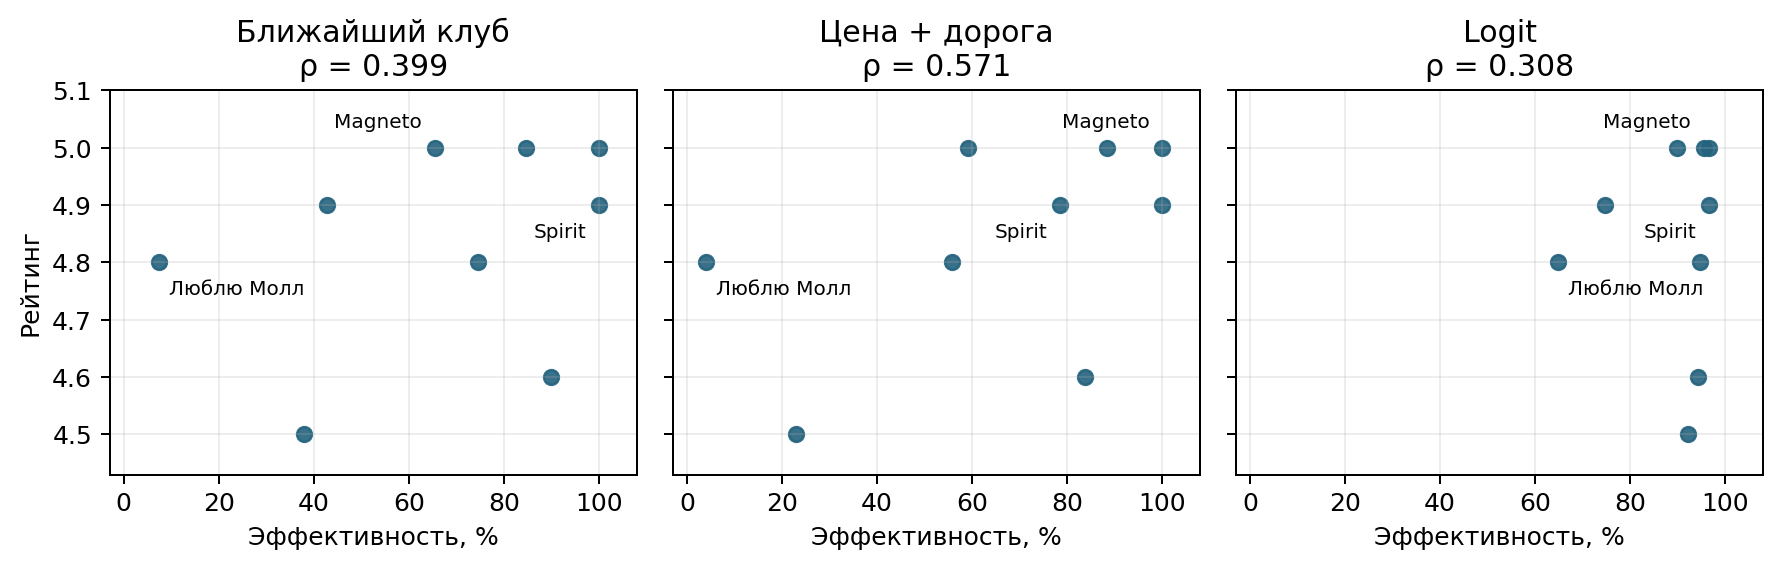
\includegraphics[width=\linewidth]{ratings_comparison.png}\caption{Рейтинг и модельная эффективность девяти клубов. $\rho$ --- корреляция Спирмена.}\end{figure}
\begin{table}[H]\centering\caption{Описательная проверка связи рейтинга и эффективности ($n=9$)}\small\begin{tabular}{lrrr}\toprule Правило выбора & $\rho$ & $p$ перестан. & $\rho$ при исключении одного\\\midrule Ближайший клуб & 0,399 & 0,281 & 0,193--0,615\\ Цена + дорога & 0,571 & 0,114 & 0,441--0,715\\ Logit & 0,308 & 0,416 & 0,158--0,546\\\bottomrule\end{tabular}\end{table}
Двусторонний перестановочный тест перебирает $9!$ перестановок при предположении обменности наблюдений. После перехода от Light к Smart корреляция центрального ценового сценария снизилась с 0,820 до 0,571; статистически убедительного подтверждения нет: выборка мала, клубы одной сети зависимы, тесты множественны, параметры сценарные. В девяти ценовых сценариях $\rho$ лежит в диапазоне от $-0,486$ до 0,818, в 27 Logit-сценариях --- от $-0,205$ до 0,915; при нулевом достижимом вкладе соответствующее $E_j$ не определено и исключается из расчёта. Рейтинги не использованы для подбора параметров.

\subsection{История открытий и необратимость размещения}
Вместо утверждения, что сегодняшняя конфигурация всегда была оптимальной, рассмотрим условный вход клубов по известным датам. Для клуба $j$ сравним $R_j^{\rm entry}$, вычисленный при наборе конкурентов на момент условного входа, с $R_j^{\rm today}$. В обоих расчётах сохраняются современные веса населения, цены, пешеходный граф и набор потенциальных площадок. Внешние клубы фиксируются; для неопределённой очередности внутри года перебираются варианты присутствия соперников. Это условная реконструкция на современной географии, не историческая оценка доходности.
\begin{table}[H]\centering\caption{Даты и условные отклонения в базовом Хотеллинге, п.п.}\small\begin{tabularx}{\linewidth}{YYrr}\toprule Клуб & Год / дата & При входе & Сейчас\\\midrule Академия Спорта & 2004? & 32,09 & 2,01\\ Территория фитнеса & 2015 & 13,84 & 0,00\\ Kometa (Raketa) & 2017 & 13,81 & 8,30\\ Z Fitness & не позднее 2019 & 4,84--7,98 & 3,50\\ СССР & не позднее 2019 & 1,20--5,69 & 7,98\\ Magneto & 2019 & 4,70--6,55 & 5,62\\ Spirit & 12.10.2021 & 0,00 & 0,00\\ DDX Экран & 26.12.2022 & 2,19 & 2,19\\ DDX Люблю Молл & 20.01.2025 & 11,90 & 11,90\\\bottomrule\end{tabularx}\end{table}
Год 2004 относится к истории Академии, а не подтверждённому открытию по нынешнему адресу; дата Kometa относится к предшественнику Raketa. Для Z Fitness и СССР годы --- верхние границы. Не реконструированы исчезнувшие клубы, смены помещений и исторические ставки аренды. Поэтому особенно большие условные оценки ранних открытий нельзя считать фактическими историческими отклонениями.

Spirit действительно открылась раньше обоих DDX, но не первой в районе. В базовой модели при фиксированном прочем окружении её доля до входа DDX составляет 18,31\%, после двух открытий --- 14,82\%, а regret равен нулю в обоих состояниях. В ценовой спецификации regret Spirit, напротив, изменяется с 1,16 до 4,94 п.п. Универсальное преимущество первого хода не подтверждается. Для СССР regret увеличивается, а для Kometa уменьшается. Возможное объяснение наблюдаемого рынка --- историческая обусловленность и издержки смены локации, но не доказанный причинный эффект очередности.

\subsection{Кейс DDX Люблю Молл: границы рынка и неоднородность услуги}
В базовом варианте чистый вклад второго клуба DDX составляет 0,95 п.п. против максимально достижимых 12,85 п.п. (эффективность 7,4\%). В модели с ценами эффективность 4,1\%, в Logit --- 64,9\%. Эти величины не являются оценками реальной рентабельности.

Проверим две альтернативные гипотезы. Во-первых, часть покупателей может посещать клуб по пути от метро. Пусть $m_i$ --- ближайший по графу вход в метро к дому $i$. Тогда альтернативная транспортная метрика
\begin{equation}
 t_{ij}^{\rm detour}=t(m_i,l_j)+t(l_j,x_i)-t(m_i,x_i).
\end{equation}
Для двух групп спроса с долями $1-\omega$ и $\omega$ используется соответственно время от дома и добавочное время маршрута от метро. В архиве имеются 14 входов двух станций. При $\omega=0,5$ эффективность Люблю Молл снижается до 3,4\%, 2,4\% и 55,6\% в трёх моделях. Гипотеза не объясняет локацию в данной спецификации.

Во-вторых, граница района может усекать спрос. В буферах 500, 1000 и 1500 м вне Марьино имеются 220, 375 и 597 архивных жилых контуров. Веса внешнего слоя пропорциональны площади, а суммарная масса задаётся сценарно относительно исходного спроса. При внешней массе 25\% в километровом буфере эффективность Люблю Молл возрастает до 17,2\%, 10,6\% и 69,1\%. Реестр внешних конкурентов неполон; это стресс-тест границы, не измерение клиентского потока из Люблино.
\begin{figure}[H]\centering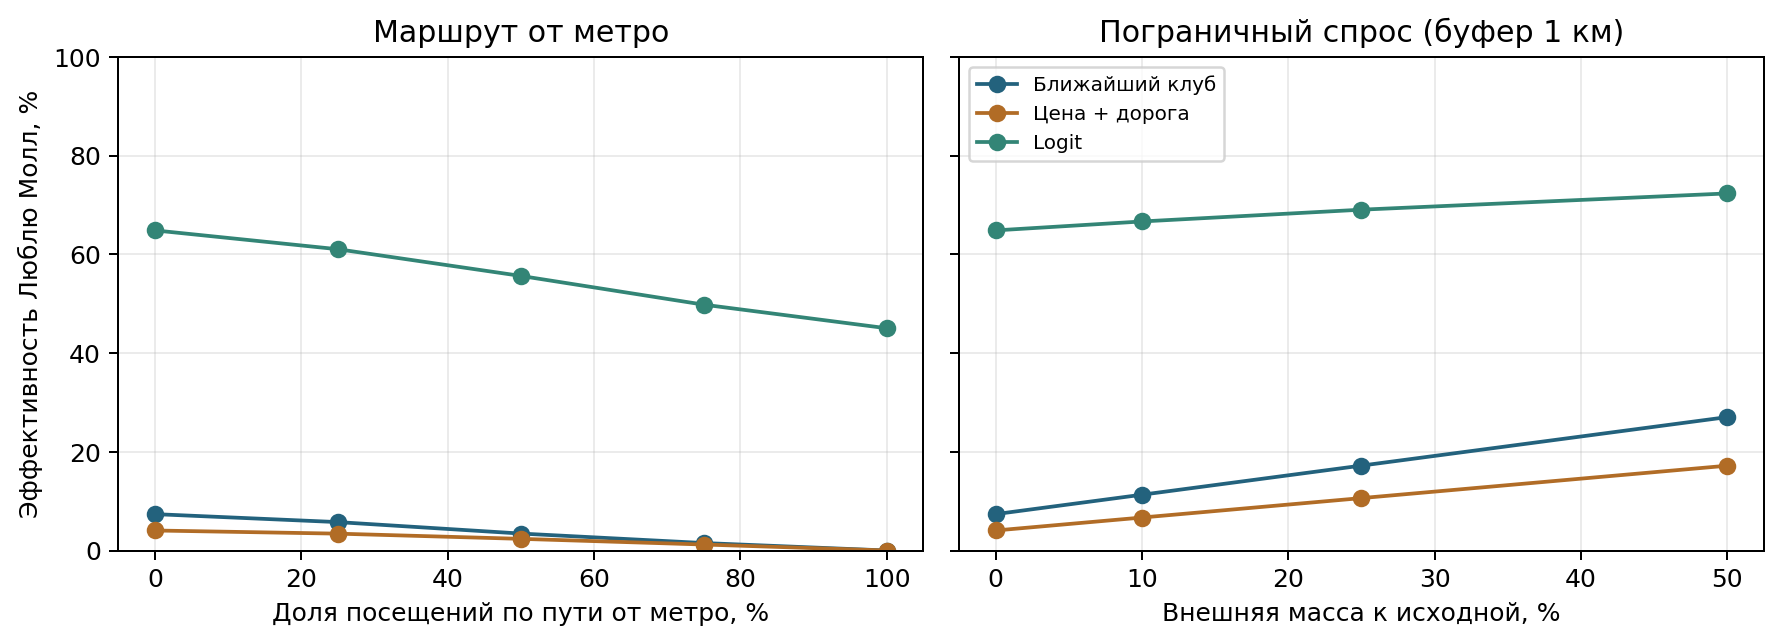
\includegraphics[width=\linewidth]{mall_sensitivity.png}\caption{Два стресс-теста для Люблю Молл. Параметры групп и внешнего спроса сценарные.}\end{figure}
Торговый центр позиционируется как обслуживающий Марьино и Люблино. Люблю Молл имеет площадь клуба около 2024 м$^2$, а тариф Infinity DDX позволяет посещать несколько клубов сети. Базовая модель одного выбранного клуба не описывает ценность мультиклубного доступа, разные площади и оборудование. В восьми пилотных тематических записях по отзывам двух клубов обнаруживаются близость к дому, переключение между филиалами, парковка, пространство и очереди. Это свидетельства существования механизмов, а не репрезентативные частоты; доказательства разгрузки Экрана нет. Полный текст отзывов и персональные данные не включены, систематическое кодирование не проводилось.

\subsection{Сопоставление инфраструктуры}
\begin{table}[H]\centering\caption{Медианные характеристики фактических и потенциальных площадок}\small\begin{tabularx}{\linewidth}{Yrr}\toprule Признак & 9 клубов & 34 альтернативы\\\midrule Жители в 10 минутах пешком & 32054 & 19518\\ До ближайшего учтённого ТЦ, м по прямой & 311 & 544\\ До входа в метро, мин по графу & 12,0 & 13,0\\ Записи магазинов и ТЦ в радиусе 300 м & 3 & 2,5\\\bottomrule\end{tabularx}\end{table}
Фактические площадки в выборке имеют более высокие медианные показатели доступного населения и коммерческой инфраструктуры. Сравнение описательное: набор альтернатив построен с исключением занятых зданий, а POI не всегда представляют уникальные организации. Наблюдение не требует машинного обучения и не устанавливает причинного влияния инфраструктуры.

\section{Консалтинговая рекомендация DDX}
\subsection{Финансовая задача}
Предлагаем выбирать не только локацию, но и решение об открытии. Пусть $m=p-c$ --- месячная маржа на дополнительного клиента, $a$ --- площадь помещения, $r$ --- арендная ставка за м$^2$, $F$ --- дополнительные ежемесячные расходы, включая при необходимости приведённые инвестиции. Тогда
\begin{equation}
 \Delta\Pi_A(z)=m\theta\Delta D_A(z)-ra-F,\qquad \max\{0,\max_{z\in L_{\rm rent}}\Delta\Pi_A(z)\}.
\end{equation}
Отказ от входа соответствует нулевому приращению прибыли. Безубыточная ставка $r^*=(m\theta\Delta D_A-F)/a$. Берём $\theta=5\%$, $m=900$ руб. (сценарная маржа, сохранена для сопоставимости), $a=1300$ м$^2$, $F=300000$ руб. в месяц. Маржа и расходы не наблюдаются. Выгода рассчитывается для всей сети, а не валового спроса нового клуба.
\begin{table}[H]\centering\caption{Финансовые пороги в лучших точках основного набора}\small\begin{tabularx}{\linewidth}{Yrrrr}\toprule Модель & Прирост, п.п. & Маржа, млн & $r^*_0$ & $r^*_{300}$\\\midrule Ближайший клуб & 12,85 & 1,581 & 1216 & 985\\ Цена + дорога & 23,35 & 2,874 & 2210 & 1980\\ Logit & 8,57 & 1,055 & 811 & 580\\\bottomrule\end{tabularx}\end{table}
Маржа приведена в млн руб./мес.; $r^*_0$ и $r^*_{300}$ --- ставки в руб./м$^2$/мес. при $F=0$ и $F=300$ тыс. руб. соответственно. Тарифы и параметры во второй и третьей строках соответствуют предыдущему разделу. Вариант «цена + дорога» даёт существенно более высокий спрос вследствие заданного преимущества DDX по цене; это не подтверждённая эластичность. Модели без ограничений загрузки могут завышать спрос. В сетке параметров Logit $r^*$ при $F=300$ тыс. варьируется от 313 до 1784 руб./м$^2$. Дополнительно в таблице \texttt{rent\_sensitivity.csv} варьируются $\theta$, маржа и $F$. Поэтому ни утверждение о гарантированной выгодности, ни утверждение о гарантированной убыточности открытия не следует из модели.
\subsection{Эмпирические ориентиры и пороги входа}
FitnessData оценивает проникновение фитнеса в Москве в 16,5\% в I квартале 2025 г. (2,18 млн клиентов); общероссийский ориентир за тот же период --- 4,85\%. Московская величина не является измерением доли жителей Марьино с действующей подпиской. Поэтому расширяем сценарии $\theta$ до 3, 5, 8, 10, 12 и 16,5\%, сохраняя 5\% как контрольный сценарий. DDX сообщает за 2025 г. о 151 клубе и 800 тыс. клиентов (около 5300 на клуб при делении агрегатов); это не оценка ёмкости зала или маржинальных затрат. В кредитном анализе АКРА фигурируют 178 клубов в сентябре 2026 г. Корпоративные показатели не идентифицируют маржу отдельного клуба.
\begin{equation}
 \theta^*(z)=\frac{ra+F}{m\Delta D_A(z)}.
\end{equation}
При аренде 1650 руб./м$^2$/мес., $a=1300$, $F=300$ тыс. и $m=900$ безубыточная доля покупателей в лучших точках составляет 7,73\% (ближайший клуб), 4,25\% (цена + дорога), 11,59\% (Logit). При $\theta=10\%$ предельные ставки соответственно 2201, 4190 и 1392 руб./м$^2$/мес. Сценарии с высокой долей покупателей и без ограничений загрузки могут давать нереалистичные объёмы: чистый прирост всей сети не равен числу клиентов нового клуба. Не следует использовать московский ориентир как точечный прогноз.
\begin{figure}[H]\centering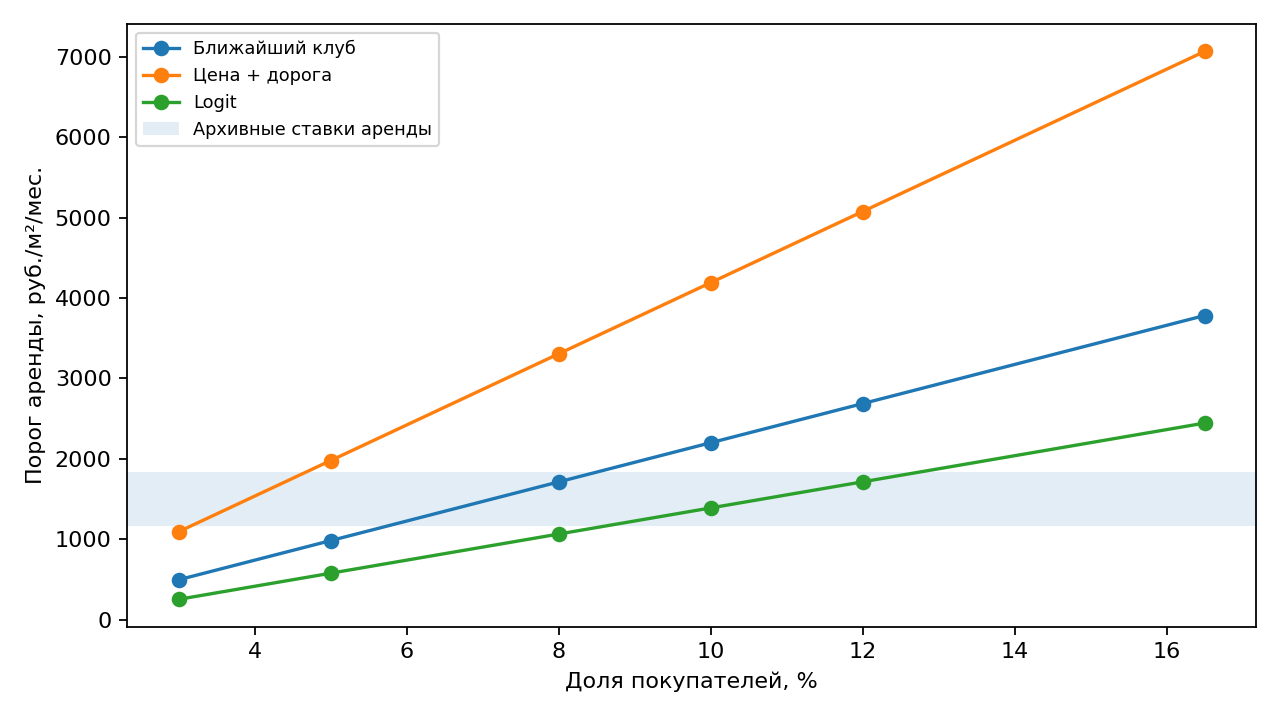
\includegraphics[width=.90\linewidth]{finance.png}\caption{Предельная арендная ставка при различных сценариях размера рынка. Маржа 900 руб., прочие расходы 300 тыс. руб.; полоса --- архивные ставки.}\end{figure}
\subsection{Наблюдаемые предложения аренды}
\begin{table}[H]\centering\caption{Архивная выборка предложений; актуальность не проверялась заново}\small\begin{tabularx}{\linewidth}{Yrrl}\toprule Адрес & Площадь, м$^2$ & Аренда, тыс. руб. & Площадь\\\midrule Перервинский б-р, 6 & 548 & 658 & Нет\\ Перерва, 54 & 600 & 700 & Нет\\ Братиславская, 18к1 & 470 & 750 & Нет\\ Братиславская, 27к1 & 636 & 827 & Нет\\ Братиславская, 30 & 955 & 1751 & Нет\\ Новочеркасский б-р, 57к2 & 1166 & 1924 & Да, не подтверждено\\\bottomrule\end{tabularx}\end{table}
Ни одно предложение не является подтверждённо доступным помещением нужного размера. Последнее подходит по площади, но ранее было снято, а теперь снова обнаружено в поисковом индексе; доступность не подтверждена. При 5\% покупателей и прочих расходах 300 тыс. руб. оно убыточно во всех трёх центральных сценариях (в варианте «цена + дорога» около 630 тыс. руб. убытка). Дополнительно найдено индексированное предложение 1297 м$^2$ за 3,243 млн руб./мес. по адресу Люблинская, 153: это ТЦ «Люблю Молл», где уже работает DDX; оно не рассматривается как независимая локация. На Новомарьинской, 20 обнаружено предложение всего 157 м$^2$. Другие блоки и инженерные параметры не подтверждены. См. \texttt{data/property\_review.csv}. Для пяти меньших объектов рассчитанные денежные значения в CSV исключительно диагностические: без моделирования вместимости их нельзя интерпретировать как бизнес-план. Выборка ставок 1167--1833 руб./м$^2$ не репрезентативна для района. В восточной зоне приоритетными объектами для проверки являются Новомарьинская, 20 и Братиславская, 21 к2. Эти адреса --- контуры зданий, а не предложения аренды. Рекомендуется запросить наличие блока 1100--1500 м$^2$, проверить инженерные условия и договор, затем сопоставить стоимость с диапазоном порогов и оценить реальный спрос. До этого не принимать обязательства об открытии.
\section{Заключение}
Главные выводы: (1) модельная концентрация существенно зависит от определения рынка, а территориальный выбор неодинаков у жителей разных кварталов; (2) сети максимизируют дополнительный спрос с учётом каннибализации; (3) ограничение географических стратегий коммерческими зданиями частично объясняет наблюдаемое размещение, особенно Spirit, но не делает весь рынок равновесным; (4) точные стратегические исходы и деньги чувствительны к предпосылкам спроса; (5) восточная зона DDX заслуживает поиска недвижимости, но инвестиционная рекомендация условна. Основные ограничения: неполный реестр конкурентов и адресных полигонов, неопределённые тарифы, неизвестные продажи, издержки и загрузка, приближённая привязка к архивной сетке. Рейтинги и история открытия дают описательные, но не причинные свидетельства. В частности, учёт цен меняет оценку Magneto; ранний вход Spirit совместим с удачным расположением, но не доказывает его причину. Пограничный спрос частично объясняет Люблю Молл, тогда как модель маршрута от метро не улучшает объяснение. Новый полный слой зданий и первичный жилищный реестр не удалось выгрузить. Проверены отдельные источники тарифов, объявлений и конкурентов, но не все записи; опрос не проводился.

\paragraph{Воспроизводимость.} \texttt{python run\_all.py} пересчитывает основной и дополнительный блоки и рисунки из комплектных данных. Выполнены 68 проверок основного и 6 дополнительного блока, включая прямое перераспределение спроса для 20 случайных локаций двух фирм, деление ничьих, контроль сохранения спроса и проверки равновесий. Это вычислительные проверки, а не эмпирическая валидация. Отчёт отражает текущий прогон; при изменении сценариев таблицы обновляются отдельно.
\section*{Источники и данные}
\small
\addcontentsline{toc}{section}{Источники и данные}
\begin{enumerate}
\item OpenStreetMap contributors. Архивный снимок OSM от 27.11.2026, граница relation/455222, адресные полигоны и матрицы расстояний; \url{https://www.openstreetmap.org/copyright}, ODbL 1.0. Слой \path{data/address_buildings.geojson} извлечён из исходного архива, OSM ID и адреса в \texttt{results/buildings.csv}.
\item DDX Fitness. Технические требования Basic: \url{https://www.ddxfitness.ru/upload/basic.pdf}. Архивная проверка требований. Сайты клубов и тарифов: ссылки в \texttt{data/clubs.csv} и \texttt{data/tariffs.csv}.
\item Объявления ЦИАН, Akula, Яндекс Недвижимости, БСКЦ и Apex: архивные ссылки и статусы в \texttt{data/properties.csv}. Дополнительная проверка отдельных предложений в \texttt{data/property\_review.csv}; доступность ни одного подходящего независимого блока не подтверждена.
\item Домпаспорт. Жилищный справочник района Марьино: \url{https://dompassport.ru/rayon/moskva/marino/}; обращение 27.11.2026. Адресные записи и число квартир в \texttt{data/housing\_registry.csv}. Вторичный источник.
\item FitnessData. Показатели проникновения фитнеса, I квартал 2025 г.: \url{https://fitnessdata.ru/tpost/j7mxvlkrc1-itogi-i-kv-2025-goda-na-rinke-fitnes-usl}. DDX Fitness, корпоративные показатели 2025 г.: \url{https://corporate.ddxfitness.ru/}. АКРА, кредитный анализ: \url{https://www.acra-ratings.ru/press-releases/7348/?lang=ru}. Сводка в \texttt{data/financial\_context.csv}.
\item Дополнительные сведения о клубах и прайс Kometa (версия 6.3, 01.09.2026): ссылки в \texttt{data/club\_review.csv}, \texttt{data/tariffs.csv}.
\item Рейтинги и даты открытия: \path{insights/data/ratings_openings.csv} содержит ссылки и оговорки по каждому клубу. Дополнительный реестр отзывов: \path{insights/data/review_pilot.csv}; Яндекс Карты, \url{https://yandex.com/maps/org/ddx_fitness/36453784004/reviews/} и \url{https://yandex.com/maps/org/ddx_fitness/36698085214/reviews/}.
\item Magneto Fitness: \url{https://magnetofitness.ru/clubs/marino/}; объявление об акции от 16.11.2026: \url{https://magnetofitness.ru/promotions-and-news/fitness-pool-spa-3742/}. DDX: \url{https://www.ddxfitness.ru/clubs/ddx-marino-ekran/}, \url{https://www.ddxfitness.ru/clubs/ddx-bratislavskaya/}; открытие Люблю Молл: \url{https://shopandmall.ru/news/ddx-fitness-zapustil-novyj-klub-plosadu-2024-kv-metra}; описание ТЦ: \url{https://love-mall.ru/about}. Подробная методология, ограничения и дополнительные источники: \path{insights/README.md}.
\item Hotelling, H. (1929). Stability in Competition. \textit{Economic Journal}, 39(153), 41--57.
\item Исходное задание курса и исходная формализация: \path{docs/assignment.pdf}, \path{docs/original_model.pdf}; происхождение данных: \path{docs/provenance.md}.
\end{enumerate}
\end{document}
